\documentclass[reqno,a4paper,12pt]{amsart}

\usepackage{amsmath,amssymb,amsthm,geometry,xcolor,soul,graphicx}
%\usepackage{array}
\usepackage{float} % 在tcolorbox中添加table (由于tcolorbox已经是一个box,因此不能直接加table)
\usepackage{subfig} % 多张图放一起
\usepackage{titlesec}
%\usepackage{enumitem}
\usepackage{enumerate}
\usepackage{lipsum}
\usepackage{listings}
\allowdisplaybreaks[4] %align公式跨页
\RequirePackage[most]{tcolorbox}
\usepackage{braket}
%\usepackage{esint} %$\varoiint$ (带圈的二重积分)
%\usepackage[colorlinks,linkcolor=red]{hyperref} %\url{}超链接
\usepackage[scheme=plain,linespread=1,punct=CCT]{ctex}% Chinese support, single line space, narrow-version SBC case punctuations
\setCJKfamilyfont{zhsong}[AutoFakeBold={2.17}]{SimSong-Regular}
\renewcommand{\songti}{\CJKfamily{zhsong}}
%\usepackage{xeCJK}
%\setCJKmainfont{Kai}
\geometry{left=0.7in, right=0.7in, top=1in, bottom=1in}

\renewcommand{\baselinestretch}{1.3}

\title{固体物理第十二次作业}
\author{董建宇 ~~ 2019511017}

\begin{document}

\maketitle

\begin{enumerate}[1.]

\item \textbf{(17.2) Law of Mass Action and Doping of Semiconductors} \\
(a) Assume that the band-gap energy $E_g$ is much greater than the temperature $k_BT$. Show that in a pure semiconductor at a fixed $T$, the product of the number of electrons $(n)$ and the number of holes $(p)$ depends only on the density of states in the valence band (through their effective masses), and on the band-gap energy. \\
$\triangleright$ Derive expressions for $n$ for $p$ and for the product $np$. You may need to use the integral $\int_0^\infty \,dx x^{1/2}e^{-x} = \sqrt{\pi}/2$. \\
(b) The band gaps of silicon and germanium are $1.1eV$ and $0.75eV$ respectively. You may assume the effective mass for silicon and germanium are isotropic, roughly the same, and are roughly .5 of the bare electron mass for both electrons and holes. (Actually the effective masses are not quite the same, and furthermore the effective masses are both rather anisotropic, but we are just making a rough estimates here.) \\
$\triangleright$ Estimate the conduction electron concentration for intrinsic (updoped) silicon at room temperature. \\
$\triangleright$ Make a rough estimate of the maximum concentration of ionized impurities that will still allow for this "intrinsic" behavior. \\
$\triangleright$ Estimate the conduction electron concentration for germanium at room temperature. \\
(c) The graph in Fig. 17.6 shows the relationship between charge-carrier concentration for a certain $n$-doped semiconductor. \\
$\triangleright$ Estimate the band gap for the semiconductor and the concentration of donor ions. \\
$\triangleright$ Describe in detail an experimental method by which these data could have been measured, and suggest possible sources of experimental error. 
\begin{figure}[h]
	\centering
	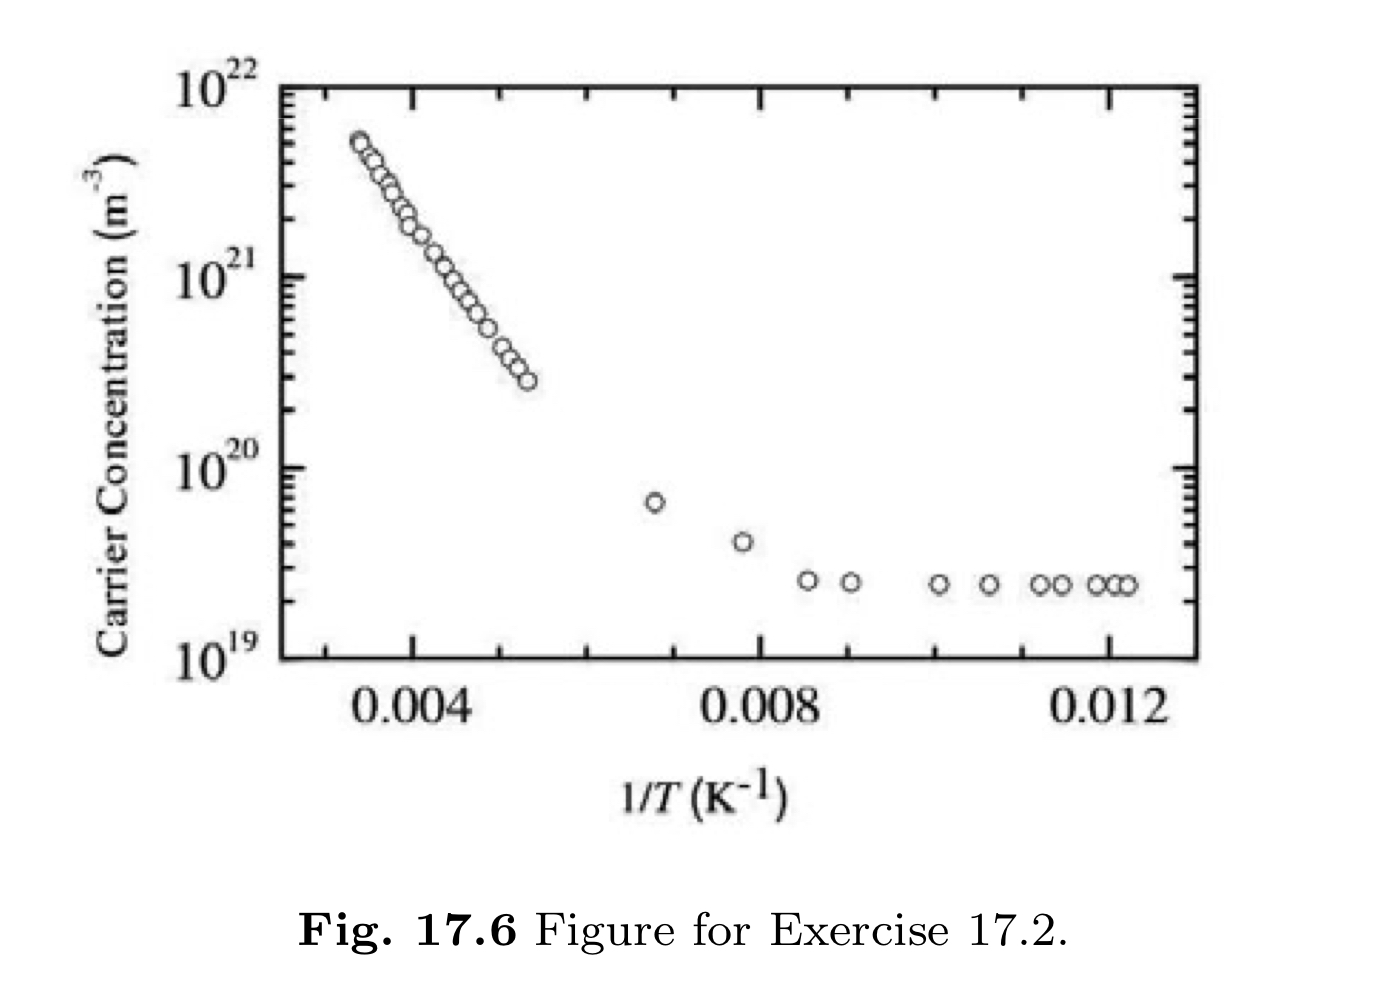
\includegraphics[width = 82mm]{17.2.jpeg}
\end{figure}
\begin{tcolorbox}[breakable, colback = black!5!white, colframe = black]
\begin{enumerate}[(a)]
\item 态密度为:
\[
	g(E) = \frac{(2m)^{3/2}}{4\pi^2\hbar^3} \sqrt{E}.
\]
则对于电子简并度为2,可以计算:
\begin{align*}
	n =& \int_{E_C}^\infty \,dE\, 2g(E-E_C) \frac{1}{e^{\beta(E-E_F)}+1} \\
	=& \frac{(2m_e^*)^{3/2}}{2\pi^2\hbar^3} \int_{E_C}^\infty \cfrac{\sqrt{E-E_C}}{e^{\beta(E-E_F)}+1} \,dE \\
	\approx& \frac{(2m_e^*)^{3/2}}{2\pi^2\hbar^3} \int_{E_C}^\infty \sqrt{E-E_C} e^{-\beta(E-E_F)} \,dE \\
	=& \frac{(2m_e^*)^{3/2}}{2\pi^2\hbar^3} e^{-\beta(E_C-E_F)} \int_0^\infty \sqrt{x}e^{-\beta x} \,dx \\
	=& \frac{1}{4}\left( \frac{2m_e^*kT}{\pi\hbar^2} \right)^{3/2} e^{-\beta(E_C-E_F)}.
\end{align*}
类似地,对于空穴简并度为2,可以计算:
\begin{align*}
	p =& \int_{-\infty}^{E_D} \,dE\, 2g(E_D-E) \left( 1 - \frac{1}{e^{\beta(E-E_F)} + 1} \right) \\
	=& \frac{(2m_p^*)^{3/2}}{2\pi^2\hbar^3} \int_{-\infty}^{E_D} \sqrt{E_D - E} \frac{e^{\beta(E-E_F)}}{1+e^{\beta(E-E_F)}} \,dE \\
	\approx& \frac{(2m_p^*)^{3/2}}{2\pi^2\hbar^3} \int_{-\infty}^{E_D} \sqrt{E_D-E} e^{\beta(E-E_F)} \,dE \\
	=& \frac{(2m_p^*)^{3/2}}{2\pi^2\hbar^3} e^{\beta(E_D - E_F)} \int_0^\infty \sqrt{x} e^{-\beta x} \,dx \\
	=& \frac{1}{4} \left( \frac{2m_p^*kT}{\pi\hbar^2} \right)^{3/2} e^{-\beta(E_F - E_D)}.
\end{align*}
则可以计算电子数目与空穴数目的乘积为:
\[
	n(T) p(T) = \frac{1}{2}\left( \frac{kT}{\pi\hbar^2} \right)^{3} (m_e^*m_p^*)^{3/2} e^{-\beta E_g}.
\]
即电子数目与空穴数目乘积只通过有效质量取决于态密度以及能隙$E_g$。

\item 
$\triangleright$ 对于本征半导体,有$n(T) = p(T) = \sqrt{n(T)p(T)} = \frac{1}{\sqrt{2}} \left( \frac{kT}{\pi\hbar^2} \right)^{3/2} (m_e^*m_h^*)^{3/4}e^{-\beta E_g/2}$在硅和锗的电子有效质量近似等于$0.5$倍自由电子质量的近似条件下,在室温下可以估算硅的导带电子浓度为:
\[
	n \approx 5.11 \times 10^{15} ~ \text{m}^{-3}
\]
$\triangleright$ 粗略估计,当参杂的电子数密度小于$10^{15}~\text{m}^{-3}$时,近似仍可以认为此半导体为本征半导体。 \\
$\triangleright$ 对于锗,在室温下导带电子数密度为:
\[
	n \approx 4.45 \times 10^{18} ~ \text{m}^{-3}.
\]

\item $\triangleright$ 在低温状态下,施主离子密度即为载流子密度,约为$2\times 10^{19} \text{m}^{-3}$。在高温状态下,载流子密度正比于$e^{-E_g/(2kT)}$,即有
\[
	\ln n \propto -\frac{E_g}{2k_B} \frac{1}{T}.
\]
由图中数据可估计斜率为:
\[
	-\frac{E_g}{2k_B} \approx \frac{\ln(1.8\times 10^{21}) - \ln(4\times 10^{20})}{0.004-0.005} \text{K} = -1504K.
\]
则能隙约为:
\[
	E_g \approx 4.153\times 10^{-20} ~ \text{J} = 0.26 ~ \text{eV}.
\]
$\triangleright$ 可以通过测量不同温度下的Hall电流进而推算出载流子浓度。得到如题中所示图线。 \\
误差可能的来源有: \\
$\bullet$ Hall元件中并不是单一载流子导电,而同时存在电子和空穴导电,因此在计算Hall系数时,应先将两不同载流子的电导率矩阵相加,进而求矩阵的逆得到电导率矩阵,从而得到Hall系数。 \\
$\bullet$ 在测量Hall电压时未精准与电流、磁场方向垂直引起的误差。 \\
$\bullet$ 在测量电压时,由于接触的影响而导致测量得到的电压并非真实的Hall电压。 

\end{enumerate}
\end{tcolorbox}

\item \textbf{(17.3) Chemical Potential} \\
(a) Show that the chemical potential in an intrinsic semiconductor lies in the middle of the gap at low temperature. \\
(b) Explain how the chemical potential varies with temperature if the semiconductor is doped with (i) donors (ii) acceptors. \\
(c) A direct-gap semiconductor is doped to produce a density of $10^{23}$ electrons/$\text{m}^3$. Calculate the hole density at room temperature given that the gap is $1.0~\text{eV}$, and the effective mass of carriers in the conduction and valence band are $0.25$ and $0.4$ electron masses respectively. Hint: use the results of Exercise 17.2.a.
\begin{tcolorbox}[breakable, colframe = black, colback = black!5!white]
\begin{enumerate}[(a)]
\item 对于本征半导体,电子密度等于空穴密度,则有:
\[
	n(T) = \frac{1}{4}\left( \frac{2m_e^*kT}{\pi\hbar^2} \right)^{3/2}e^{-\beta(E_C-E_F)} = p(T) = \frac{1}{4}\left( \frac{2m_p^*kT}{\pi\hbar^2} \right)^{3/2}e^{-\beta(E_F-E_D)}
\]
在低温极限下,费米能近似等于化学势,则可以解得:
\[
	\mu = \frac{1}{2}(E_C+E_D) - \frac{3}{4}kT\ln\left( \frac{m_e^*}{m_p^*} \right) \approx \frac{1}{2}(E_C+E_D).
\]
即在低温极限下本征半导体的化学势在能隙中间。

\item 对于参杂的半导体,电子密度不等于空穴密度,但是有:
\[
	\frac{n(T)}{p(T)} = \left( \frac{m_e^*}{m_p^*} \right)^{3/2} e^{-\beta(E_C+E_D-2E_F)}.
\]
则可以解得:
\[
	E_F = \frac{1}{2}(E_C+E_D) + \frac{1}{2}kT\ln\left( \frac{n}{p} \right) + \frac{3}{4} kT \ln\left( \frac{m_p^*}{m_e^*} \right).
\]
假设电子与空穴的有效质量相同,则上式中第三项为0。\\
(i)对于施主填充,有$n>p$,则化学式近似为费米能级为:
\[
	\mu = \frac{1}{2}(E_C+E_D) + \frac{1}{2}kT\ln\left( \frac{n}{p} \right) > \frac{1}{2}(E_C+E_D).
\]
同时,随着温度的升高化学势升高。 \\
(ii)对于受主填充,有$n<p$,则化学势近似为费米能级为:
\[
	\mu = \frac{1}{2}(E_C+E_D) + \frac{1}{2}kT\ln\left( \frac{n}{p} \right) < \frac{1}{2}(E_C+E_D).
\]
同时,随着温度的升高化学势降低。

\item 由17.2.a可知,电子数密度与空穴数密度乘积为:
\[
	n(T)p(T) = \frac{1}{2} \left( \frac{kT}{\pi\hbar^2} \right)^3 (m_e^*m_p^*)^{3/2} e^{-\beta E_g}.
\]
由题目可知,$n = 10^{23}~\text{m}^{-3}$, $T = 300~K$, $E_g = 1.0 ~ \text{eV}$, $m_e^* = 0.25m_e$, $m_p^* = 0.4m_e$,可以计算对于本征半导体,$n = p$时电子数密度为:
\[
	n = \sqrt{np} = 2.51 \times 10^{16} \text{m}^{-3}.
\]
注意到本征半导体中电子数密度远小于参杂导致的电子数密度,则可以计算空穴数密度为:
\[
	p = 3.16\times 10^9 \text{m}^{-3}.
\]

\end{enumerate}
\end{tcolorbox}

\item \textbf{(18.1) Semiconductor Quantum Well} \\
(a) A quantum well is formed from a layer of GaAs of thickness $L$ nm, surrounded by layers of $\text{Ga}_{1-x}\text{Al}_x\text{As}$ (see Fig. 18.2). You may assume that the band gap of the $\text{Ga}_{1-x}\text{Al}_x\text{As}$ is substantially larger than that of GaAs. The electron effective mass in GaAs is $0.068~m_e$ whereas the hole effective mass is $0.45~m_e$ with $m_e$ the mass of the electron. \\
$\triangleright$ Sketch the shape of the potential for the electrons and holes. \\
$\triangleright$ What approximate value of $L$ is required if the band gap of the quantum well is to be $0.1$ eV larger than that of GaAs bulk material? \\
(b) *What might this structure be useful for?
\begin{tcolorbox}[breakable, colback = black!5!white, colframe = black]
\begin{enumerate}[(a)]
\item $\triangleright$ 束缚在量子井中的载流子可以用量子力学中无限深势井近似,其具有分立的能级,对于电子而言,能量为:
\[
	E_{e,m} = E_C + \frac{1}{2m_e^*}\left( \frac{m\pi\hbar}{L} \right)^2.
\]
近似的,对于空穴而言,能量为:
\[
	E_{h,m} = E_D - \frac{1}{2m_h^*}\left( \frac{m\pi\hbar}{L} \right)^2.
\]
其中m为正整数,可以绘制草图如下:
\begin{figure}[H]
	\centering
	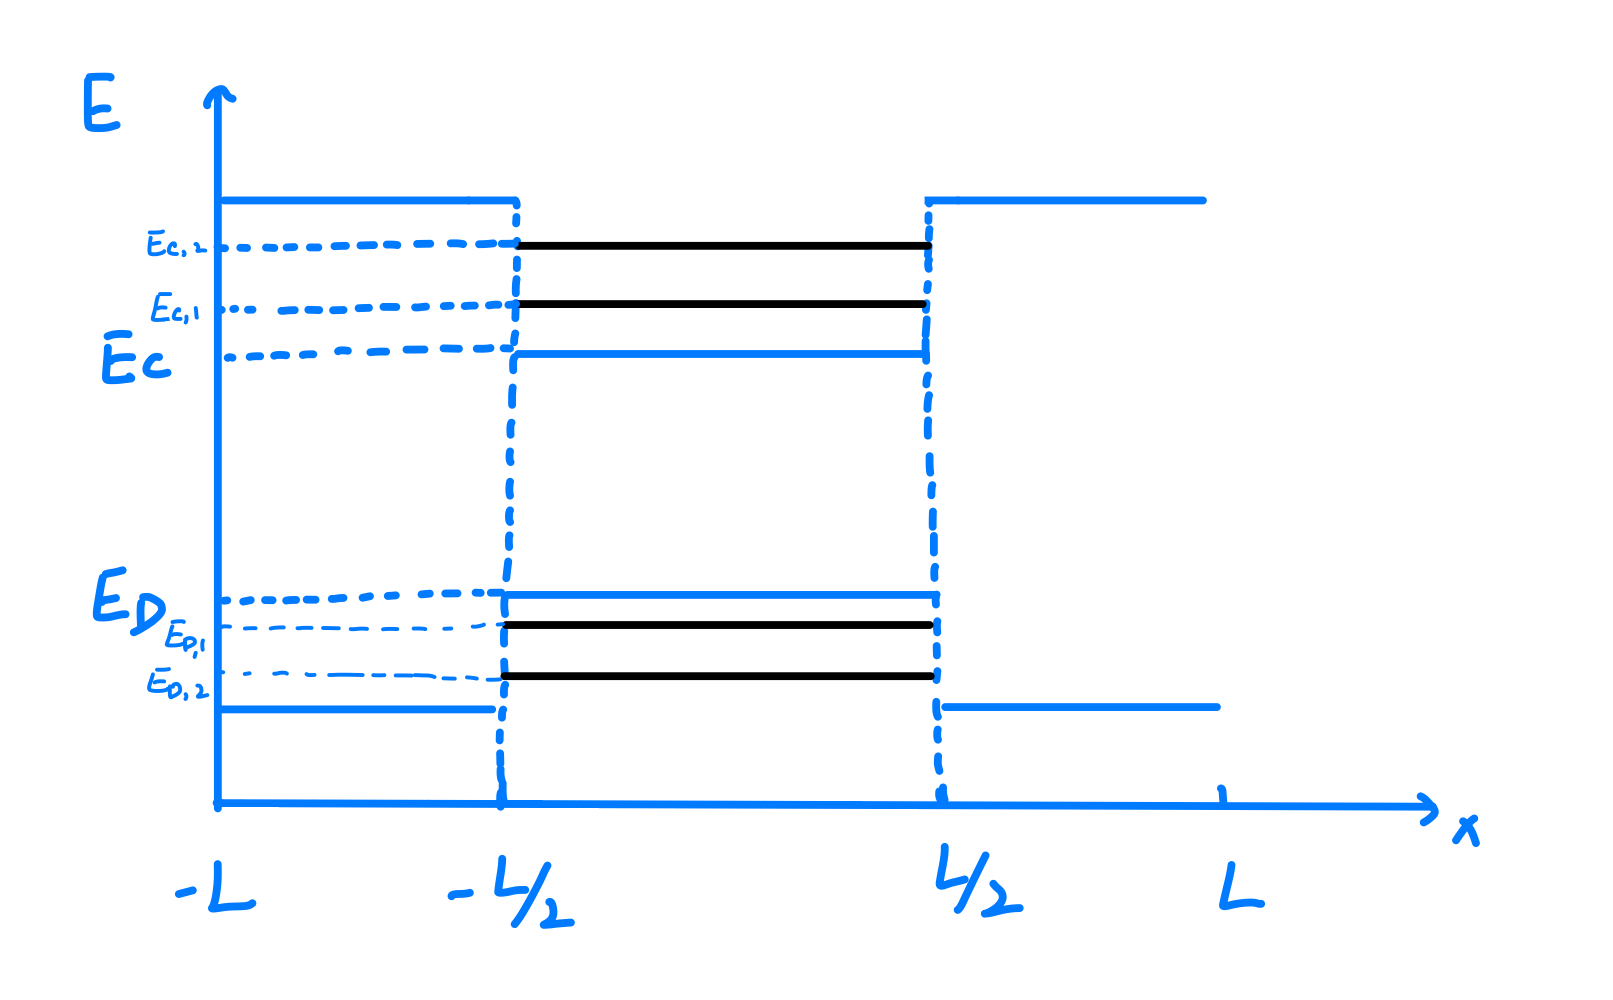
\includegraphics[width = 120mm]{18.1.jpeg}
	\caption{电子与空穴的能级草图}
\end{figure}
$\triangleright$ 当量子井的带隙比砷化镓带隙大0.1eV时,有:
\[
	(E_{e,1} - E_{h,1}) - (E_C - E_D) = \frac{\pi^2\hbar^2}{2L^2} \left( \frac{1}{m_e^*} + \frac{1}{m_h^*} \right) = \Delta E_g.
\]
带入数据可计算得:
\[
	L = 7.97 \times 10^{-9}\text{m} = 7.97 \text{nm}.
\]

\item 可以通过调节$\text{Ga}_{1-x}\text{Al}_x\text{As}$中$Al$的参杂量$x$来调节量子井深度,同时,可以通过调节GaAs厚度来调节能隙大小,从而可以使用该种材料制成任意输出频率的激光。

\end{enumerate}
\end{tcolorbox}

\item \textbf{(18.3) $p-n$ Junction*} \\
Explain the origin of the depletion layer in an abrupt $p-n$ junction and discuss how the junction causes rectification to occur. Stating your assumptions, show that the total width $w$ of the depletion layer of a $p-n$ junction is: 
\[
	w = w_n+w_p
\]
where 
\[
	w_n = \left( \frac{2\epsilon_r\epsilon_0 N_A\phi_0}{eN_D(N_A+N_D)} \right)^{1/2}
\]
and a similar expression for $w_p$ Here $\epsilon_r$ is the relative permittivity and $N_A$ and $N_D$ are the acceptor and donor densities per unit volume, while $\phi_0$ is the difference in potential across the $p-n$ junction with no applied voltage. You will have to use Poisson's equation to calculate the form of $\phi$ given the presence of the ion charges in the depletion region. \\
$\triangleright$ Calculate the total depletion charge and infer how this changes when an additional voltage $V$ is applied. \\
$\triangleright$ What is the differential capacitance of the diode and why might it be useful to use a diode as a capacitor in an electronic circuit?
\begin{tcolorbox}[breakable, colback = black!5!white, colframe = black]
\textbf{耗尽区的来源}:当p型半导体与n型半导体相互接触时,n型半导体导带中较多的电子倾向于转移到p型半导体空的价带中从而降低体系的能量,同时在n型半导体接触面附近留下正离子,在p型半导体附近留下负离子,从而形成了从n型半导体指向p型半导体的电场,这又会驱动电子从p型电导体向n型半导体流动,当这两种作用达到平衡时,宏观上就会存在一段区域不存在载流子,这就是耗尽区。 \\
\textbf{整流的原理}:d电子从n型半导体扩散到p型半导体引发的扩散电流满足如下正比关系:
\[
	I_{diff} \propto \exp(-\beta E_g).
\] 
同时,内建电场引发的电流满足:
\[
	I_{drift} \propto \exp(-\beta (E_g-eV)).
\] 
其中$V$为外加偏压,此时总电流为:
\[
	I = I_{drift} - I_{diff} \propto \exp(-\beta E_g) (\exp(\beta eV) - 1).
\]
注意到当电压为正向时,电流较大;但当施加反向偏压时,电流会很小。这就是整流效果。 \\
选取$n$型参杂半导体与$p$型参杂半导体中间位置为坐标原点,$x<0$区域为$n$型参杂;$x>0$区域为$p$型参杂,则Possion方程为:
\[
	\nabla^2 \phi(x) = \frac{\rho}{\epsilon_r\epsilon_0}.
\]
选取坐标为$x=0$为势能零点,解为:
\[
	\phi(x) = \left\{ \begin{array}{ll}
		-\cfrac{eN_D}{2\epsilon_r\epsilon_0}x^2 + C_1 x, & x<0; \\
		\cfrac{eN_A}{2\epsilon_r\epsilon_0}x^2 + C_2 x, & x>0.
	\end{array} \right.
\]
在耗尽区边界处电场为0,则可以确定待定参数满足方程:
\begin{align*}
	&\left. \frac{d\phi}{dx} \right\vert_{x=-w_n} = \frac{eN_D}{\epsilon_r\epsilon_0}w_n + C_1 = 0, \\
	&\left. \frac{d\phi}{dx} \right\vert_{x=w_p} = \frac{eN_A}{\epsilon_r\epsilon_0}w_p + C_2 = 0.
\end{align*}
则有:
\[
	\phi(x) = \left\{ \begin{array}{ll}
		-\frac{eN_D}{2\epsilon_r\epsilon_0}(x^2+2\omega_nx), & x<0; \\
		\frac{eN_A}{2\epsilon_r\epsilon_0}(x^2-2\omega_px), & x>0. 
	\end{array} \right.
\]
则两端电势差为:
\[
	\phi_0 = \phi(-\omega_n) - \phi(\omega_p) = \frac{e}{2\epsilon_r\epsilon_0} (\omega_n^2N_D + \omega_p^2N_A).
\]
由于总电荷量为0,则有:
\[
	\omega_nN_D = \omega_pN_A.
\]
联立上式可得:
\begin{align*}
	w_n =& \left( \frac{2\epsilon_r\epsilon_0 N_A\phi_0}{eN_D(N_A+N_D)} \right)^{1/2}, \\
	w_p =& \left( \frac{2\epsilon_r\epsilon_0 N_D\phi_0}{eN_A(N_A+N_D)} \right)^{1/2}.
\end{align*}

$\triangleright$ 耗尽区单位面积的电荷为:
\[
	q = eN_D\omega_D = \left( \frac{2\epsilon_r\epsilon_0 e N_DN_A \phi_0}{N_A+N_D} \right)^{1/2}.
\]
若施加外电压$V$,则只需要将电势差$\phi_0$改为$\phi_0+V$,得:
\[
	q = eN_D\omega_D = \left( \frac{2\epsilon_r\epsilon_0 e N_DN_A (\phi_0+V)}{N_A+N_D} \right)^{1/2}.
\]

$\triangleright$ 二极管的微分电容为:
\[
	C = \frac{\partial q}{\partial V} = \left( \frac{2\epsilon_r\epsilon_0 e N_DN_A}{N_A+N_D} \right)^{1/2}(\phi_0+V)^{-1/2}.
\]
即二极管的电容随所加电压变化而变化,也就意味着可以通过调整电压从而实现二极管电容的调整。
\end{tcolorbox}

\item \textbf{(19.1) $\ddagger$ Atomic Physics and Magnetism} \\
(a) Explain qualitatively why some atoms are paramagnetic and others are diamagnetic with reference to the electronic structure of these materials. \\
(b) Use Hund's rules and the Aufbau principle to determine $L$, $S$, and $J$ for the following isolated atoms: \\ 
\text{} \hspace{1em} (i) Sulfur (S), atomic number = 16 \\
\text{} \hspace{1em} (ii) Vanadium (V), atomic number = 23 \\
\text{} \hspace{1em} (iii) Zirconium (Zr), atomic number = 40 \\
\text{} \hspace{1em} (iv) Dysprosium (Dy), atomic number = 66
\begin{tcolorbox}[breakable, colback = black!5!white, colframe = black]
\begin{enumerate}[(a)]
\item 有些原子自旋轨道耦合使得总角动量$J$不等于0,从而出现磁矩,再外加磁场的条件下,磁矩会趋向于与磁场方向同向,从而在宏观上表现出磁矩,这就是顺磁性。 \\
对于满壳层原子,总角动量为零,再外加磁场的条件下,由于电子在做拉莫尔进动,产生反向磁场,从而在宏观上体现出抗磁性。

\item 
\begin{enumerate}[(i)]
	\item S原子的电子排布为$[Ne]3s^23p^4$,则轨道角动量为$L=1$,自旋角动量为$S=1$,电子超过半满,则总角动量为$J=L+S=2$。
	
	\item V原子的电子排布为$[Ar]3d^34s^2$,则轨道角动量为$L=3$,自旋角动量为$S=3/2$,电子小于半满,则总角动量为$J=L-S=3/2$。
	
	\item Zr原子的电子排布为$[Kr]4d^25s^2$,则轨道角动量为$L=3$,自旋角动量为$S=1$,电子小于半满,则总角动量为$J=L-S=2$。
	
	\item Dy原子的电子排布为$[Xe]4f^{10}6s^2$,则轨道角动量为$L=6$,自旋角动量为$S=2$,电子小于半满,则总角动量为$J=L+S=8$。
\end{enumerate}

\end{enumerate}
\end{tcolorbox}


\end{enumerate}

\end{document}